% !TeX root = ../main.tex

\chapter{相关研究综述}
本章主要介绍在时间序列异常检测和复杂系统根因定位方向的相关工作。
\label{cha:related:work}
\section{时间序列异常检测技术}
本节首先介绍传统得到基于统计方法的工作,然后介绍目前用深度学习做异常检测的代表性工作,最后引出当前深度学习方法评估存在的问题。
\label{sec:intro:time}
\subsection{基于统计的方法}
时间序列异常检测是一个很经典的问题。传统方法主要基于统计,最常用也最高效的是基于3$\sigma$原则,基于历史的数据分布来确定当前数据的合理波动范围。它假设数据分布满足正态分布,因此不在$(\mu - 3\sigma,\mu + 3\sigma)$范围内的数据极有可能是异常值。但实际数据可能不符合正态分布的假设,具体使用的偏离倍数也很难统一。另一种常用的是ARIMA\footnote{Autoregressive Integrated Moving Average model,差分整合移动平均自回归模型}\cite{contreras2003arima}方法,通过前一段的时间的数据来预测下一个时刻的数据,然后通过比较预测值和真实值的差异来判断异常的发生,适用于平稳、少突降和突增的数据,但该方法有7个参数需要确定,并且不同的时间序列数据难以找到一套自动化的流程来确定参数。

\subsection{基于深度学习的方法}
近年来,随着人工智能技术的发展,越来越多的深度学习技术被用到了这一领域。而鉴于异常检测这一问题的特殊性:标签难以获得以及难以穷尽所有的异常,所以得到所有的有标数据然后做一个二分类的有监督学习分类器这一方法不具备可行性,因此目前在异常检测领域无监督方法还是主流,也就是用正常的数据训练,在这个过程中学习到正常数据的模式,然后根据异常不符合正常数据的模式这一特性将测试数据中的异常区分出来。而用无监督的方法做异常检测也有基于预测、重构等思路,以下介绍各个思路的代表性工作。

\subsubsection{基于预测}

Malhotra\cite{malhotra2015long}首次将LSTM用于时间序列异常检测这一领域,用LSTM来预测未来一段时间内的数据,并且假设预测误差符合高斯分布,在训练时用最大似然估计\cite{white1982maximum}来得到高斯分布的参数,测试时则通过预测数据与真实数据的误差从高斯分布中采样得到的概率大小来判断异常是否发生异常。

Hundman\cite{DBLP:conf/kdd/HundmanCLCS18}用同样的方式做预测,然后对预测误差使用EWMA\footnote{Exponentially Weighted Moving-Average,指数加权滑动平均}平滑,然后提出了一个基于统计的动态阈值来进行异常的判断,而不需要对误差作符合高斯分布的假设。

但总体而言,基于预测然后靠预测误差来判断异常的方法在面对到突变较多的时间序列数据如图~\ref{fig:bad:predict}时表现很差,因为该类数据本身就是无法预测的。

\begin{figure}[htbp]
    \centering
    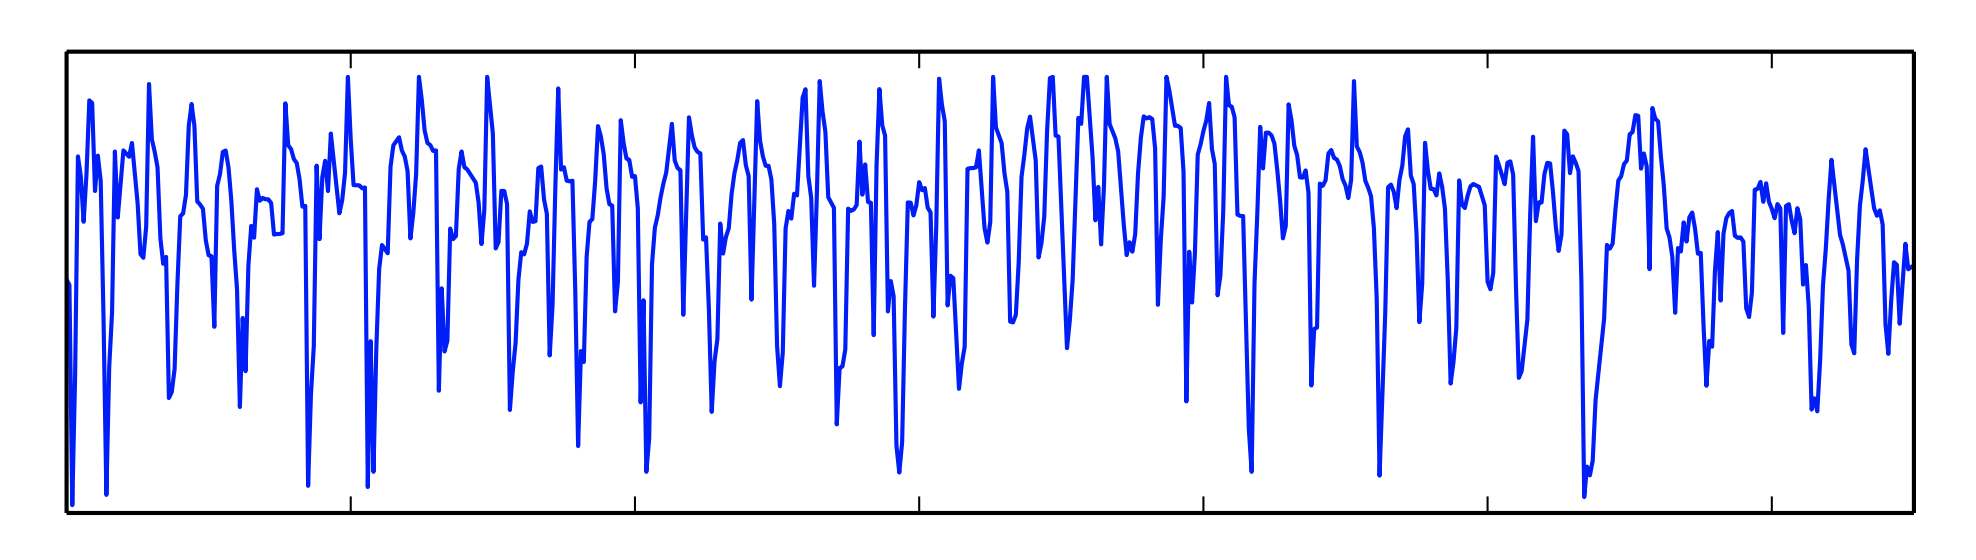
\includegraphics[width=\textwidth]{bad_predict.png}
    \caption{无法预测的时间序列数据\cite{malhotra2016lstm}}
    \label{fig:bad:predict}
  \end{figure}

\subsubsection{基于重构}

基于重构的深度学习方法来做异常检测的思路是用自编码器模型对正常数据进行无监督的训练,而对异常数据进行重构就会显现出较大的重构误差。

An\cite{an2015variational}利用VAE\footnote{Varitional AutoEncoder,变分自编码器}来做异常检测,其模型结构如图~\ref{fig:vae:model}所示,通过对正常数据分布的参数建模而不是直接对值建模。在AE中,其潜在变量是由编码器的确定性映射表示得到的,而VAE使用的概率编码器则能在采样过程中考虑潜在变量的可变性,因此这扩展了AE的表达能力,因为即使正常数据与异常数据可能共享相同的平均值,其可变性也可能不同。作者在此基础上引入了重构概率来代替重构误差进行异常检测。

\begin{figure}[htbp]
    \centering
    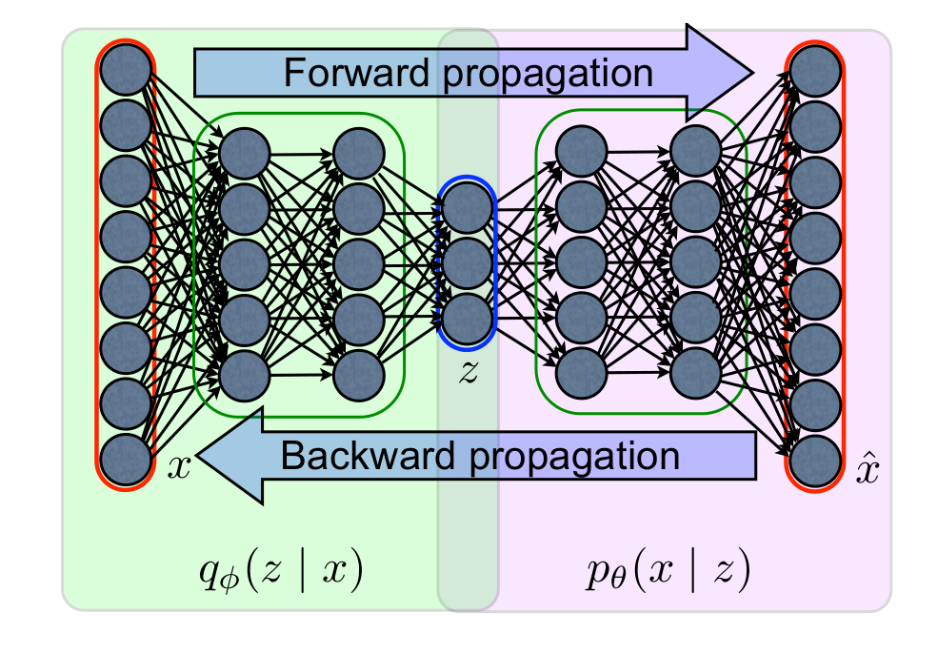
\includegraphics[width=\textwidth]{vae_model.png}
    \caption{VAE模型结构示意图\cite{an2015variational}}
    \label{fig:vae:model}
  \end{figure}

\subsubsection{重构与预测相结合}
Malhotra\cite{malhotra2016lstm}提出了一个将预测与重构结合起来的模型LSTM-ED,其模型结构如图~\ref{fig:lstm:ed}所示,通过LSTM模型将一段时间内的数据编码成一个定长变量,再作为另一个LSTM模型倒序着将原序列解码出来,最后根据重构出来的数据与原数据的误差用和\cite{malhotra2015long}类似的方法来判断异常。

\begin{figure}[htbp]
    \centering
    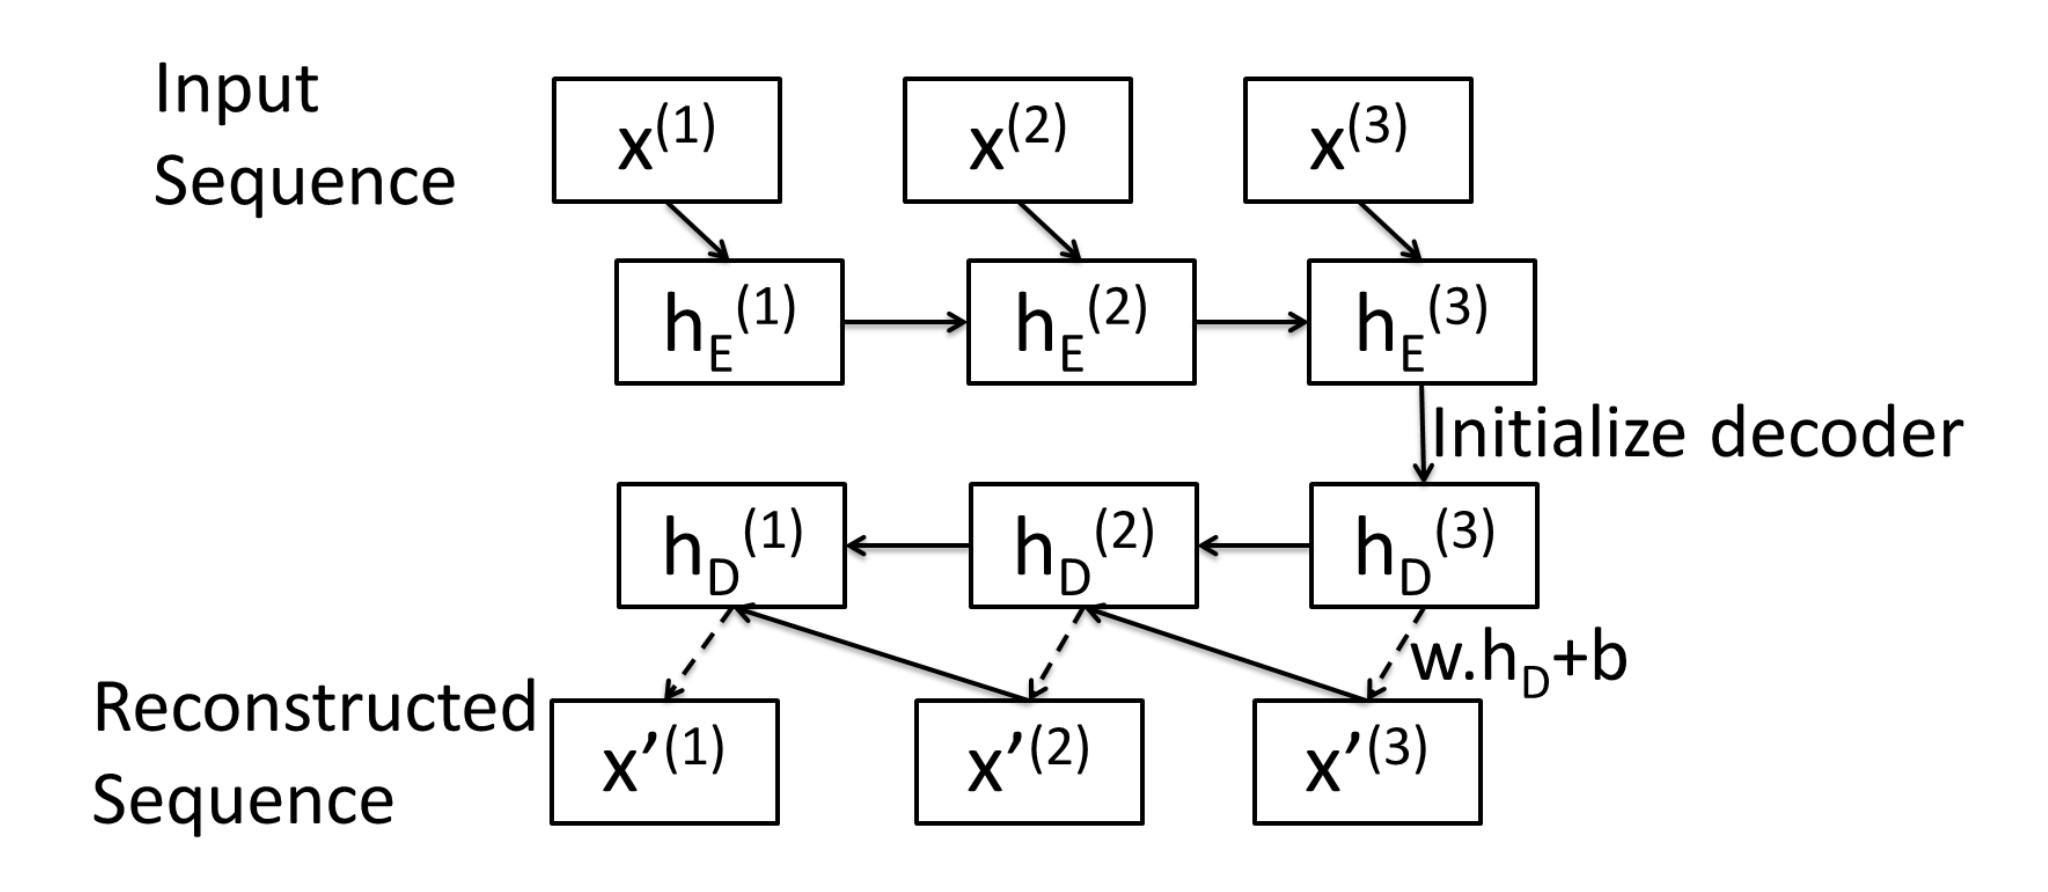
\includegraphics[width=\textwidth]{lstm_ed.png}
    \caption{LSTM-ED模型结构示意图\cite{malhotra2016lstm}}
    \label{fig:lstm:ed}
  \end{figure}


% 除了预测和重构之外,Ruff\cite{ruff2018deep}用神经网络来实现OC-SVM\footnote{One-Class Support Vector Machine,一分类支持向量机}来解决传统OC-SVM在面临高维数据时表现差的问题;



%最近,Park\cite{park2018multimodal}将LSTM和VAE结合起来,规避了VAE本身并不是一个时序模型的特点,将其用于机器人的传感器数据异常检测上并获得了不错的效果;

%Su\cite{su2019robust}则进一步考虑了VAE中随机变量的时序性的特点,在ServerMachineDataset数据集下实现了目前为止最好的结果。


\subsubsection{传统方法深度化}

OC-SVM\cite{DBLP:journals/tdsc/WatsonSMMH16}是一种用于异常检测的分类器,其不同于一般的SVM做一个多分类问题而是做的单一分类问题。由于异常检测中获取不到完整的异常数据让分类器去完整的学习异常类别的特征,因此使用OC-SVM来学习正常数据这一类别的特征,将所有正常数据映射到一个球里,如果新数据用相同的映射不在球里则认为是异常,这个映射通常用核函数来完成,但该方法在面对到比较高维的数据则准确度较低,因为这个映射也就是核函数的形式难以选取,因此Ruff\cite{ruff2018deep}选择用神经网络来自动地学习该映射。

GMM\footnote{Gaussian Mixture Model,高斯混合模型}\cite{reynolds2009gaussian}可以看作是由$K$个单高斯模型组合而成的模型,当有了正常数据分布的GMM参数后,同样可以评估数据的出现概率来判断异常,但该方法在面临到高维数据时也效果很差,{Zong\cite{zong2018deep}则将AE与传统的GMM模型结合起来提出了DAGMM模型,其结构如~\ref{fig:deep:autoencoder}所示分为Compression Network和Estimation Network,前者用来将数据压缩到较低维度,而后者则用来估计GMM的参数,两者在训练过程中相互影响,最终完成一个端到端的异常检测任务。

\begin{figure}[htbp]
  \centering
  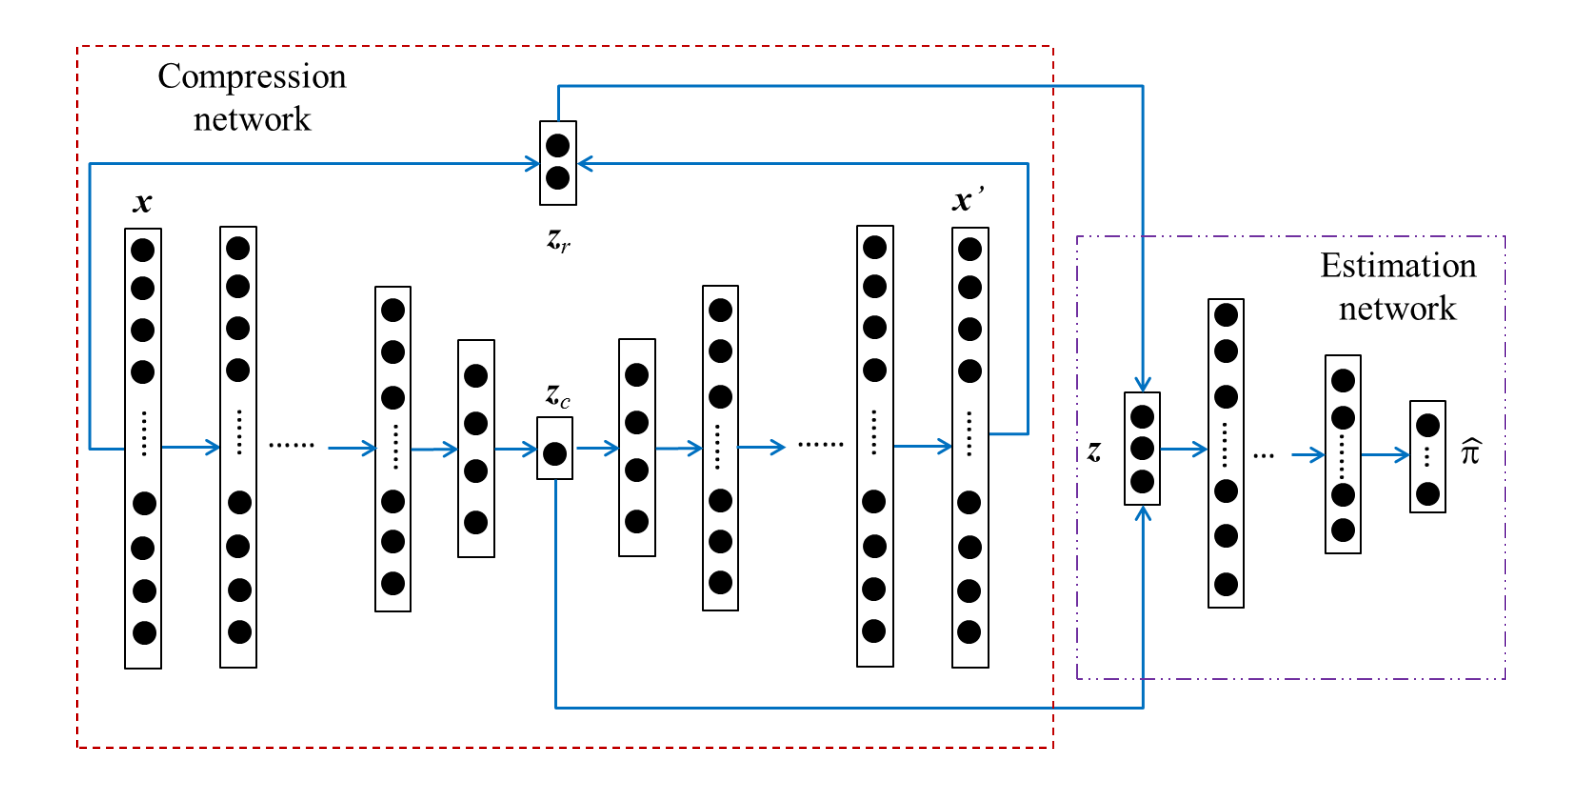
\includegraphics[width=\textwidth]{deep_autoencoder.png}
  \caption{DAGMM模型结构示意图\cite{malhotra2016lstm}}
  \label{fig:deep:autoencoder}
\end{figure}

可以看到将传统方法深度化,主要是用深度学习的方法来降维,从而应对原方法在面对到高维数据时失效的问题。

\subsection{时间序列异常检测模型的评估}
时间序列异常检测的评估不同于单点异常检测评估。因为其前后有相关性,如图~\ref{fig:range:eval}所示。Hundman\cite{DBLP:conf/kdd/HundmanCLCS18}使用的方法是将一整段异常作为一个异常来算$Precision$和$Recall$,但如何定义一段异常是否被检测到也缺乏一个标准;Xu\cite{xu2018unsupervised}提出了一种简单的调整的方式,认为一段异常中只要有一个点被检测到那么整段都认为被检测到,然后在这个基础上重新计算$Precision$和$Recall$,但该方法也存在不够准确的方法,而且往往评价指标会虚高。因为对于一段很长的异常来说,模型只要能够检测到最为异常的那一个点,就能获得整段的分数。Tatbul\cite{tatbul2018precision}则系统地研究了这个问题,并且提出了一种新的针对时间序列的$Precision$和$Recall$的计算方式,将预测异常和真实异常都表示为区间的方式,综合考虑到预测异常与真实异常的相交的大小、位置、唯一性带来的不同影响,为时间序列异常检测提供了一个较为合理的评价指标。
\begin{figure}[htbp]
    \centering
    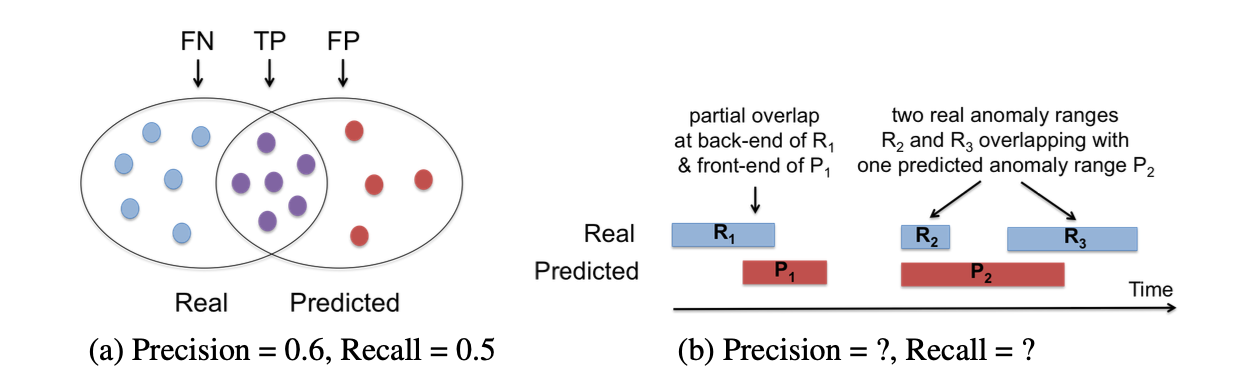
\includegraphics[width=\textwidth]{range_eval.png}
    \caption{时间序列异常检测的评估与传统异常检测的不同\cite{tatbul2018precision}}
    \label{fig:range:eval}
  \end{figure}

\section{复杂系统中的根因定位}

在云网络中的根因定位工作方面,难点在于如何将异常之间的传播关系表示出来并根据传播关系追溯到根因。

Lin\cite{lin2016automated}提出了异常传播路径的概念,将多点之间的关联边分为水平边和竖直边,其中虚拟机和虚拟机之间因为服务调用会发生异常的传播,这种边为水平边,而坐落在同一个物理机上的虚拟机之间会因为争夺资源互相影响,这种边则是竖直边,在有了异常传播图的基础上到所有异常点的距离之和就作为评判一个点是根因的依据。该方法的问题在于没有设置边权,实际上边与边之间发生异常传播的概率也是不同的;

Weng\cite{weng2018root}则针对公共云中的多级服务调用场景在此Lin\cite{lin2016automated}的基础上做出了改进,在图中对边的类型进行了区分并且引入了边权,通过计算时间序列数据之间的相关性来作为边权:如果该节点的性能指标曲线与服务调用耗时曲线的相关性越高,那么就认为在该节点上产生的异常越有可能通过服务调用传播给其他相邻节点;在计算根因时Weng选择了用随机游走来更真实地模拟异常传播,实现了更加准确的根因分析。

Wang\cite{DBLP:conf/ccgrid/WangXMLPWC18}在云网络中进行了根因分析的工作,通过类似的方法来建图,在根因分析时使用了二阶随机游走的方法,在进行下一步的节点选择时不仅要考虑到当前所处节点,还考虑了上一个所处的节点。Wu\cite{wu2020microrca}则在微服务场景下进行了根因定位的工作,在定位这一步上使用了Personal PageRank\cite{page1999pagerank}来更加高效和准确地计算根因。

以往的方法大都是将时间序列数据之间的相关性作为边权来构建异常传播图,在此基础上来考虑异常的传播,很少将时间序列数据异常检测的结果充分应用起来。因此本文将二者结合起来,提出了一个新的构图方式,在此基础上运用随机游走的算法得到根因。

\section{小结}
通过分析已有的相关工作,可以看出一方面,在时间异常检测领域,深度学习的方法缺乏一个统一的标准来评价,因此本文希望设计一个通用的框架,内部使用合理的评价方式对已有的算法或者新算法进行性能、速度等各方面综合的评价;另一方面,在根因定位上以往的方法多与异常检测的联系不是那么密切,本文希望能够将异常检测的结果作为异常传播图的一部分,在此基础上进行随机游走来获得根因定位的结果。

